\begin{abstract}
Орчин цагт интернэт сүлжээ хүмүүсийн амьдралын салшгүй нэг хэсэг болж түүнийгээ дагаад бүхий л мэдээ мэдээллийг интернэт дэх нэмэлт эх сурвалжуудаас авдаг болсон. Аливаа зүйлс томрох тусам найдвартай, чанартай зүйлстэй зэрэгцэн худал хуурмаг зүйлс их тархдаг билээ. Үүнтэй ижлээр хүмүүс интернэт дэх хэт олон эх сурвалжууд дунд төөрч, хэрэгцээгүй мэдээлэл унших, түүнийгээ бусдад хуваалцаж бусдыг болон өөрсдийгөө үргэлжлүүлэн хохироосоор байна. Үүнээс авч үзвэл интернэт хэрэглэгчид мэргэжлийн хүмүүсийн цуглуулсан чанартай агуулгатай эх сурвалжуудыг хялбар, нэгдсэн байдлаар харах, мөн өөрөө эх сурвалжуудаа цуглуулж бусдад хуваалцах шаардлага тулгарч байна.

	\setcounter{secnumdepth}{0}

  \section{Зорилго}
	Мэдээллийн эх сурвалжуудаа нэгтгэж бусдад хуваалцах, бусдын цуглуулсан эх сурвалжуудыг хялбар байдлаар харах, үнэлгээ өгөх боломжтой веб апп бүтээж интернэт хэрэглэгчдийн нэмэлт эх сурвалж олох явцыг хялбаршуулахаар зорьж байна.

	\section{Зорилт}
	Уг веб аппыг хөгжүүлэхдээ дараах үе шатын дагуу ажиллана.
	\begin{enumerate}
		\item Хэрэглэгчийн үндсэн шаардлагуудыг тодорхойлох
		\item UX судалгаа хийж хэрэглэгч суурьтай хялбар интерфейс дизайн гаргах
		\item Ашиглах технологийг онол болон практик дээр суурилж судлах, 
		\item Системийн архитектурыг зохион байгуулж бэлдэх
		\item Гаргасан баримт бичиг дээрээ тулгуурлаж хөгжүүлэлтээ хийх
		\item Эцсийн хэрэглэгчиддээ зориулж бүтээгдэхүүн болгон гаргах
	\end{enumerate}
	
	\section{Сэдэв сонгох үндэслэл}

	2022 оны 4-р сарын байдлаар дэлхийн нийт хүм амын 63.1 хувь буюу ойролцоогоор 5 тэрбум хүн интернэт сүлжээг хэрэглэдэг ба үүнээс 4.7 тэрбум хүн буюу 94 хувь нь өдөр тутмын амьдралдаа сошиал сүлжээг ашиглаж бусадтай харилцах, мэдээ мэдээллээ авах хэрэгцээгээ хангадаг байна \footnote{Дэлхийн интернэт хэрэглэгчдийн судалгаа: \url{https://www.statista.com/statistics/617136/digital-population-worldwide/}}. Өөрөөр хэлбэл дэлхийн хүн амын талаас их хувь нь хэвмэлэл биет материал, телевиз, радиогоос гадна нэмэлтээр интернэт дэх веб холбоосуудаар дамжин нэмэлт мэдээллээ авдаг гэсэн үг билээ.
	
	Миний хувьд сошиал сүлжээ ашиглан уг сэдэвтэй холбоотой судалгааг\footnote{Эх сурвалжтай холбоотой судалгаа: \url{https://docs.google.com/spreadsheets/d/1CfVnHT29pkBiL0JBv7bXiKtOxERQfTzt0PmOaQ-mcd0/edit?usp=sharing}} 58 интернэт хэрэглэгчдээс авсан бөгөөд тэдгээрт тулгарсан асуудлууд болон хариултуудыг дүгнэж үзвэл

	\begin{figure}[h]
		\centering
		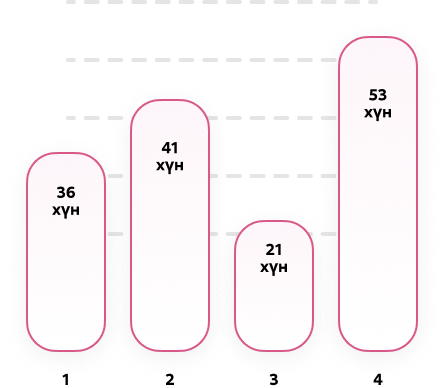
\includegraphics[width=5cm]{images/statistic.png}
		\caption{Интернэт хэрэглэгчдээс авсан судалгааны үр дүн}
		\label{fig:results}
	\end{figure}

	\begin{enumerate}
		\item Маш олон хуурамч мэдээллүүдэд өртдөг - 36 хүн
		\item Өөрт хэрэгтэй мэдээллээ олоход цаг их зарцуулдаг - 41 хүн
		\item Сэдвийнхээ хүрээнд өөрийн олж авсан эх сурвалжуудын тоонд сэтгэл хангалуун бус байдаг - 21 хүн
		\item Ном, зурагтаас илүү интернэт ашиглан мэдээллээ авдаг - 53 хүн
	\end{enumerate}

	гэсэн хариу гарсан. Иймд эдгээр болон бусад хэрэглэгчдэд шаардлагатай зөвхөн эх сурвалжуудаа олж авах, бусдад хуваалцах боломжтой сошиал платформыг бүтээсэн нь зөв гэж үзсэн тул уг сэдвийг сонгон хөгжүүлж байна.

	\section{Ач холбогдол}
	Уг платформыг бүтээснээр миний хувьд бүтээгдэхүүнийг эхнээс нь дуусах хүртэлх хөгжүүлэлтийн үе шатуудтай танилцах, түүнийгээ практикаар хэрэгжүүлэх боломж бүрдэнэ. 

	Мөн бүтээгдэхүүн болгон гаргаж хэрэглээнд нэвтрүүлснээр дээр дурдсан асуудлыг тодорхой хэмжээнд багасах боломжтой гэж үзэж байна. Маш олон төрлөөр хэрэглэх боломжтой ба жишээ нь их сургуулийн багш оюутнууддаа зориулж сэдвийн хүрээнд нэмэлт материал бэлдэхдээ интернэт сүлжээнд байрласан унших ёстой судалгааны ажил, үзэх ёстой бичлэг, дагаж хийх ёстой практик хичээлүүдийнхээ веб холбоосуудыг хялбар байдлаар нэгтгэж, хуваалцах боломж бүрдэх юм. Мөн багш нь өөрийн сонирхдог сэдвийн хүрээнд бусдын оруулсан эх сурвалжуудтай танилцах боломжтой. 
	\setcounter{secnumdepth}{2}
	% \thispagestyle{plain}

\end{abstract}
